%version of 08-10-18

\chapter{RECURRENCES}
\label{ch:Recurrences}

This chapter is devoted to derive and solve Linear Recurrences.

While we have discussed already discussed the use of linear
recurrences in Section ***CHECK REFERENCE  %~\ref{sec:linear-recurrences-1}, 
we derive the underlying mathematics in this section

\section{The Master Theorem}
\label{sec:mesterTheorem}

\subsection{A simplified form}

By the time the reader has reached this paragraph, she has the
mathematical tools necessary to prove and apply what is called {\it
  The Master Theorem for Linear Recurrences} \cite{CLRS}.  This level
of mathematical preparation should be adequate for most
early-undergrad courses on data structures and algorithms, as well for
for analyzing a large fraction of the algorithms that she is likely to
encounter in daily activities.

\begin{theorem}[The Master Theorem for Linear Recurrences]
\label{thm:master-thm}
\index{The Master Theorem for Linear Recurrences}
Let the function $F$ be specified by the following linear recurrence.
\begin{equation}
\label{eq:Lin-Recur:start}
F(n) \ = \ \left\{
\begin{array}{cl}
a F(n/b) + c & \mbox{for } n \geq b \\
c & \mbox{for } n < b
\end{array}
\right.
\end{equation}
Then the value of $F$ on any argument $n$ is given by
\begin{equation}
\label{eq:Lin-Recur:solve}
\begin{array}{lclll}
F(n) & = & (1 + \log_b n)c &  & \mbox{if } a=1 \\
     &   &                 &  & \\
     & = &
  {\displaystyle
  \frac{1-a^{\log_b n}}{1-a} \ \approx \ \frac{1}{1-a}
  }
 &  & \mbox{if } a<1 \\
    &   &                  & & \\
    & = &
  {\displaystyle
\frac{a^{\log_b n} -1}{a-1}
  }
 & & \mbox{if } a>1
\end{array}
\end{equation}
\end{theorem}

\begin{proof}
In order to discern the recurring pattern in
(\ref{eq:Lin-Recur:start}), let us begin to ``expand'' the specified
computation by replacing occurrences of $F(\bullet)$ as mandated in
(\ref{eq:Lin-Recur:start}).
\begin{equation}
\label{eq:Lin-Recur:expand}
\begin{array}{lcccc}
F(n) & = & a F(n/b) + c & & \\
     & = & a \left( a F(n/b^2) + c \right) + c
             & = & a^2 F(n/b^2) + (a+1)c \\
     & = & a^2 \left( a F(n/b^3) + c \right) + (a+1)c
             & = & a^3 F(n/b^3) + (a^2+a+1)c \\
     &   & \vdots & & \vdots \\
     & = & 
{\displaystyle
\left(a^{\log_b n} + \cdots +a^2+a+1 \right) c
} & &
\end{array}
\end{equation}
The segment of (\ref{eq:Lin-Recur:expand}) ``hidden'' by the vertical
dots betokens an induction that is left to the reader.  Equations
(\ref{eq:geom-sum:b>1}) and (\ref{eq:geom-sum:b<1}) now enable us to
demonstrate that (\ref{eq:Lin-Recur:solve}) is the case-structured
solution to (\ref{eq:Lin-Recur:start}).  \qed
\end{proof}

\subsection{A more complicated (but still regular) form}

We present in this section a more general recurring pattern:

\begin{equation}
\label{eq:Lin-Recur:general}
F(n) \ = \ \left\{
\begin{array}{cl}
a F(n/b) + f(n) & \mbox{for } n > b \\
1 & \mbox{for } n = b
\end{array}
\right.
\end{equation}

Let us first solve the case where function $f$ is linear, i.e. in the simplified form $f(n) = n$.
We also assume for clarity that $n$ is a power of $b$. 

We proceed as previously by replacing the successive occurrences of $F$:

\begin{equation}
\label{eq:Lin-Recur:expand}
\begin{array}{lcccc}
F(n) & = & a F(n/b) + n & & \\
     & = & a \left( a F(n/b^2) + n/b \right) + n
             & = & a^2 F(n/b^2) + (a.n/b+n) \\
     & = & a^2 \left( a F(n/b^3) + n/b^2 \right) + (a.n/b+n)
             & = & a^3 F(n/b^3) + (a^2/b^2+a/b+1)n \\
     &   & \vdots & & \vdots \\
     & = & 
{\displaystyle
\left(a^{\log_b n}F(1) + \sum_{i=0,\log_b (n)-1} (a/b)^i \right) n
} & &
\end{array}
\end{equation}

\begin{figure}[htb]
\begin{center}
       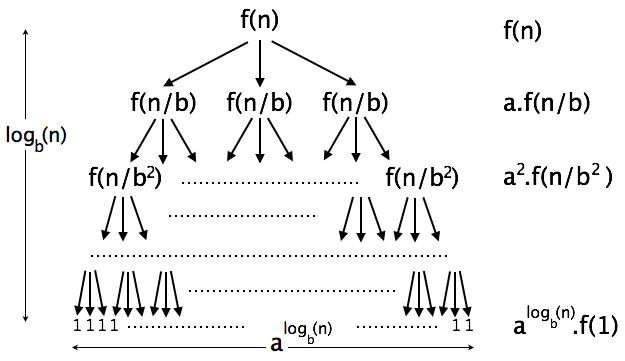
\includegraphics[scale=0.4]{FiguresMaths/MasterTheoremgeneral}
\caption{{\it Development of the computations. Summation on the right.}
\label{fig:masterTheorem}}
\end{center}
\end{figure}

Fig.~\ref{fig:masterTheorem} illustrates these computations.
The second term corresponds to a geometric sequence.

The interpretation is that if $a$ is larger than $b$, $F(n)$ is dominated by the first term while if it is smaller, the second term dominates.
The problem is perfectly balanced between the iterations when $a=b=2$, we obtain $F(n) = n.log_2(n)$. 


\section{The Fibonacci Recurrence and its Kin}
\label{sec:Fiboacci-plus}

\subsection{The Fibonacci sequence}

Leonardo of Pisa, ``the son of Bonaccio''

In the original problem introduced by Leonardo of Pisa (Fibonacci) in the middle age, 
Fibonacci numbers are the number of pairs of rabbits that can be produced at the successive generations. 
Starting by a single pair of rabbits and assuming that each pair produces a new pair of rabbits 
at each generation during only two generations. 
\bigskip

\noindent
{\bf Definition.}
Given the two numbers $F(0) = 1$ and $F(1) = 1$, 
the Fibonacci numbers are obtained by the following expression: 

$F(n+1)= F(n)+F(n-1)$.
\bigskip

%\begin{figure}[h]
%\begin{center}
%        \includegraphics[scale=0.4]{FIGmaths/DefFibo}
%        \caption{Principle of the Fibonacci progression}
%        \label{doublesum}
%\end{center}
%\end{figure}


Notice that it is a special case of $u_{n+1} =\alpha.u_{n} + \beta.u_{n-1}$ for $\alpha=\beta=1$.
\bigskip

There is a strong link between these numbers as the diagonal and the Pascal triangle:

As shown in Figure~\ref{fig:FiboPascal}, Fibonacci numbers can be obtained by summing up the successive numbers of the diagonals.
The explanation is illustrated in Figure~\ref{fig:FiboPascalExplanation}: a diagonal is obtained by summing the two previous ones and the two first start at 1. 
%Another way to write this relation is by the following expression:
%$F_n = binomial (n,0,1 ...)$

\begin{figure}[h]
\begin{center}
        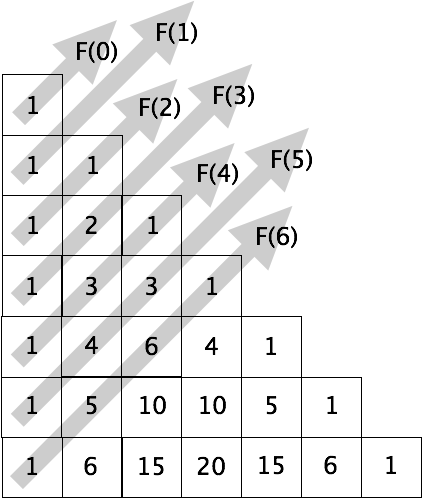
\includegraphics[scale=0.4]{FiguresMaths//FiboPascal1}
        \caption{Obtaining Fibonacci numbers are the diagonals of the Pascal triangle justified to the left. }
        \label{fig:FiboPascal}
\end{center}
\end{figure}

\begin{figure}[h]
\begin{center}
        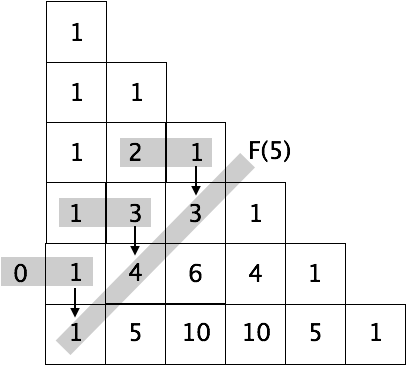
\includegraphics[scale=0.4]{FiguresMaths//FiboPascal2}
        \caption{Each term of the diagonal is obtained by summing up both previous ones.}
        \label{fig:FiboPascalExplanation}
\end{center}
\end{figure}


\section{Some recurrences on Fibonacci numbers}

%Fibonacci numbers are defined by the following numerical progression:
%$n \geq 2$ $F(n) = F(n-1) + F(n-2)$, $F(0)=F(1)=1$.
These numbers have nice properties, like the following one. 

\noindent \textbf{Property.} 
\label{prop:FiboSum}
$F(n+2) =1+ \sum_{k=0}^{n} F(k) $
\bigskip

\noindent The proof is by induction.

\begin{itemize}
\item
The \textbf{basis case} (for $n=2$) is true since $F(2) = 1+F(0)$.

\item
\textbf{Induction step:} Let assume the property holds at rank $n$ for $F(n+2)$ and compute $F(n+3)$:

Apply the definition of Fibonacci numbers: $F(n+3) = F(n+1)+F(n+2)$ 

Replace the last term by the recurrence hypothesis: $F(n+2) = 1+\sum_{k=0}^{n} F(k)$

Thus, $F(n+3) = F(n+1) + 1+ \sum_{k=0}^{n} F(k)  = 1+\sum_{k=0}^{n+1} F(k)$
\end{itemize}

\subsection{Computing the product of two consecutive Fibonacci numbers}

\noindent \textbf{Property.} 
\label{prop:FiboSumConsecutive}
$F(n).F(n-1)= \sum_{k=0}^{n-1} F(k)^2$ (for $n \geq 1$)

\begin{itemize}

\item The relation  
can be proved very easily by the geometric argument shown in Fig.~\ref{fig:fibosquare}). 

\begin{figure}[h]
\begin{center}
        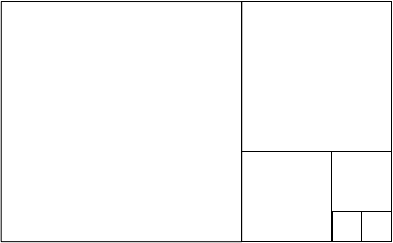
\includegraphics[scale=0.5]{FiguresMaths//Fiboembedded}
        \caption{Geometric interpretation of the relation $F(n).F(n-1)$.}
        \label{fig:fibosquare}
\end{center}
\end{figure}

\item
Another proof is by induction.

\begin{itemize}
\item
The \textbf{basis case} is to check $F(0).F(1) = F(0)^2$, which is true.

\item
\textbf{Induction step:} Let assume this property holds at rank $n$ and compute $F(n+1).F(n)$.

Apply the definition of $F(n+1)$:

 $F(n+1).F(n) =  (F(n)+F(n-1)).F(n) = F(n)^2 +  F(n).F(n-1)$
 
 Apply now the induction hypothesis to this last term:
 
 $F(n+1).F(n) = F(n)^2 + \sum_{k=0}^{n-1} F(k)^2 = \sum_{k=0}^{n} F(k)^2$.
 \end{itemize}

\end{itemize}

\subsection{Another property dealing with squares}

We will show the following property by two different methods

\noindent \textbf{Property.} 
\label{prop:FiboEmbedded}
$F(n+2)^2 = 4.F(n).F(n+1) + F(n-1)^2$ for $n \geq 2$.


The geometrical proof is obtained as depicted in Fig.~\ref{fig:fibosquareembedded} for computing $F_{n+2}^2$.

\begin{figure}[h]
\begin{center}
        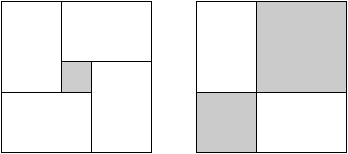
\includegraphics[scale=0.5]{FiguresMaths//FiboSquares}
        \caption{Geometric interpretation for computing $F_{n+2}^2$.}
        \label{fig:fibosquareembedded}
\end{center}
\end{figure}

Let remark that this figure might be adapted to show several properties using various decompositions of the squares and rectangles.

Another proof uses directly the definition of the Fibonacci numbers:

%$F_{n+1} + F_{n}$

$F(n+2)^2 = (F(n+1) + F(n))^2 $

$= F(n+1)^2+2.F(n+1).F(n)+F_{n}^2$

$= 4.F(n+1).F(n) - 2.F(n+1).F(n) + F(n+1)^2 + F(n)^2$

$= 4.F(n+1).F(n) + (F(n+1) - F(n))^2$

Again, using the definition of $F(n+1)$ into the square, we get the expected result:

$F(n+2)^2 = 4.F(n+1).F(n) + F(n-1)^2$


\subsection{Cassini's identity}

\noindent \textbf{Property. (Cassini's identity)} 
\label{prop:cassini}
$F(n-1).F(n+1) = F(n)^2 + (-1)^{n+1}$ for $n \geq 1$.


The proof by induction is as follows:

\begin{itemize}
\item 
The \textbf{basis case} is straightforward since $F(0).F(2) = 2$ and $F(1)^2 +1 = 2$.

\item
The \textbf{induction step} is proved assuming the Cassini's identity holds at rank $n$.

Apply the definition of $F(n+2)$:
 
$F(n).F(n+2) = F(n) (F(n+1)+F(n)) = F(n)^2 + F(n).F(n+1))$

Replace the last term using the recurrence hypothesis:

$F(n)^2 = F(n-1).F(n+1) - (-1)^{n+1} =F(n-1).F(n+1) + (-1)^{n+2} $

Thus,
$F(n).F(n+2) = F(n).F(n+1) + F(n-1).F(n+1) + (-1)^{n+2} = F(n+1) (F(n) + F(n-1)) + (-1)^{n+2}$ 

Apply again the definition of Fibonacci sequence $F(n) + F(n-1) = F(n+1)$, we obtain:

$F(n).F(n+2) = F(n+1)^2 + (-1)^{n+2}$
\end{itemize}


The previous result (Cassini's identity) can be used for a geometrical paradox (one of the favorite puzzle of Lewis Carroll).
Consider a chess board and cut it into 4 pieces as shown in figure~\ref{paradox}, then reassemble them into a rectangle.
%Interpret this paradox.
%
\begin{figure}[h]
\begin{center}
\label{paradox}
       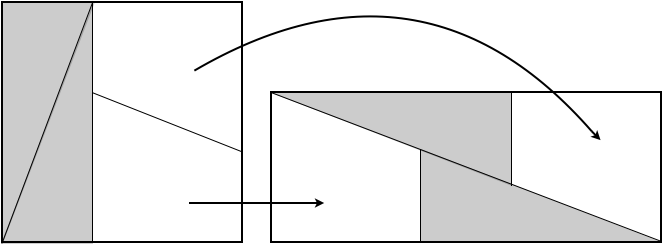
\includegraphics[scale=0.4]{FiguresMaths//FiboParadox.png}
              \caption{Construction of the rectangle after splitting the $8 \times 8$ square
              in two right $8$ by $3$ triangles and two polytopes.}
        \label{fig:FiboParadox}
\end{center}
\end{figure}

The surface of the square is $F(n)^2$ while the rectangle is $F(n+1).F(n-1)$.
In Fig.~\ref{fig:FiboParadox}, the Cassini identity is applied for $n=5$, $F(5)=8$. 
On one side, we obtain a surface of $8 \times 8 = 64$, but $13 \times 5 = 65$ on the other side!
What's wrong?

The paradox comes from the wrong representation of the diagonal of the rectangle which does not coincide with the hypothenuse
of the right triangles of sides $F(n+1)$ and $F(n-1)$.
In other words, it always remains (for any $n$) an empty space (corresponding to the unit size of the basic square of the chess board).
The greater $n$, the better the paradox because the deformation of the surface of this basic square becomes more tiny. 


%\subsection{Using Fibonacci numbers}
%
%$F(n)$ is the number of paths from node $1$ to $n$ in the following family of graphs of figure~\ref{fibograph}. 
%
%\begin{figure}[h]
%\begin{center}
%        \includegraphics[scale=0.4]{../FIGmaths/FiboGraph.pdf}
%        \caption{Counting paths from node $1$ to node $n$ ($n=7$)}
%        \label{fibograph}
%\end{center}
%\end{figure}
%%Show how this number is related to Fibonacci's numbers.
%%\item Find a closed form for the sum of consecutive Fibonacci numbers.

\subsection{Combinatorial interpretation of Fibonacci numbers}

Let count the number of binary vectors whose components donot have two consecutive $1$. Call $F(n)$ this number.

Look at the last bit of the binary representation of $n$.

\begin{itemize}
\item
If it is equal to $1$ thus, the previous bit (in position $n-1$ should be $0$.
In this first case, the number the number is equal to $F(n-2)$
\item
If the last bit is $0$, the number is $F(n-1)$
\end{itemize}
Thus, $F(n) = F(n-1) + F(n-2)$
\bigskip

This alternative view of looking at the Fibonacci numbers allows us to establish some elegant proofs.
This is for instance the case for Property~\ref{prop:FiboSum}. 

\subsection{Toward a close form of the current term of the sequence}

In this section, we present the general methodology for determining the close form of $F(n)$,
that is an direct expression that only depends on $n$ and not on the other terms of the sequence.
The characteristic equation of $F(n+2) - F(n+1) - F(n) =0$ is:

$x^2 - x - 1 = 0$

Let determine its discriminant: $\Delta = 5$.
Since it is positive, this equation has two distinct roots:

$\Phi = \frac{1+\sqrt{5}}{2}$ and $\Phi' = \frac{1-\sqrt{5}}{2}$

The first one $\Phi$ is known as the \textit{golden ratio}. 

The general term $F(n)$ is equal to $a.\Phi^n + a'.\Phi'^n$ where $a$ and $a'$ are determined by two particular values $n=0$ and $n=1$:

$F(n)= \frac{1}{\sqrt{5}} ((\frac{1+\sqrt{5}}{2})^n - (\frac{1-\sqrt{5}}{2})^n)$

\subsection{Relatives of the Fibonacci sequence}

The Lucas' sequence...

A natural question is what happens if we change the first ranks of the sequence keeping the same recurrence pattern?
It has been studied by the french mathematician Edouard Lucas, starting at 2 and 1. 
For some reasons that will be clarified later, the sequence is shifted (we take the convention $L(-1)=2$).

{\Denis do you agree with this shift of the sequence? it simplifies several proofs...}
\bigskip

\noindent
{\bf Definition.}
Given the two numbers $L(0) = 1$ and $L(1) = 3$, 
all the other Lucas numbers are obtained by the same progression as Fibonacci: 
$L(n+1) = L(n)+L(n-1)$.
\bigskip

n: 0, 1, 2, 3, 4, 5, 6, 7, 8, 9, ...

F(n): 1, 1, 2, 3, 5, 8, 13, 21, 34, 55, ...

L(n): 1, 3, 4, 7, 11, 18, 29, 47, 76, 123, ...
\bigskip

There are several interesting links with Fibonacci numbers.

In particular, we established at the beginning of this chapter in Property~\ref{prop:FiboSum} that
$F(n+2) = 1+ \sum_{k=0}^{n} F(k)$. 

We have similarly: $L(n+2) = 1+ \sum_{k=-1}^{n} L(k)$ since the basic step of the induction is still valid: $L(2) = L(-1 )+L(0) +1 = 2+1+1 = 4$.
%Actually, it will be true for all the progressions where $u_1=1$.
\bigskip

We can also easily show that the Lucas number of order $n$ is the sum of two Fibonacci numbers:

\noindent \textbf{Property. } 
\label{prop:Lucas1}
$L(n) = F(n-1)+F(n+1)$ for $n \geq 1$
\medskip


The proof is by induction as follows.

\begin{itemize}
\item
The \textbf{basis case} (for $n=2$) is true since $L(1) = 3 = F(2) + F(0) = 2+1$.

\item
\textbf{Induction step:} Let assume the property holds at all ranks $k \leq n$ and compute $L(n+1)$:

Apply the definition of Lucas' numbers: $L(n+1) = L(n)+L(n-1)$

Apply the induction hypothesis on both terms:

 $L(n+1) = F(n+1)+F(n-1)+F(n)+F(n-2)$
 
Apply now the definition of Fibonacci numbers for $F(n+1) + F(n) = F(n+2)$  and $F(n-1) + F(n-2) = F(n)$
and replace them in the previous expression:

$L(n+1) = F(n+2)+F(n)$
which concludes the proof.

%
\end{itemize}
\medskip

Notice that using a similar proof, we obtain $L(n) = F(n+2)+F(n-2)$. 
However, the generalization it is no more true for the further terms.
The interested reader can easily prove:

$L(n) = \frac{1}{2} (F(n+3)+F(n-3))= \frac{1}{3} (F(n+4)+F(n-4))$, and so on.
\medskip

Another interesting expression is the following.

\noindent \textbf{Property. } 
\label{prop:Lucas2}
$F(n+1) = \frac{1}{2} (F(1).L(n) + F(n).L(1))$


\medskip
The proof comes from direct arithmetic manipulations:

$2.F(n+1) = F(n+1) +  F(n+1) =  F(n+1) + F(n) + F(n-1)$

$= L(n) + F(n) $

$= F(1).L(n) + F(n).L(1)$
\medskip


The previous property can be extended for any $m>1$ as follows:

\noindent \textbf{Property. } 
\label{prop:Lucas3}
$2.F(n+m) = F(m).L(n) + F(n).L(m)$

The proof is left to the reader.

\bigskip

\noindent \textbf{Corollary:} Another interesting expression is
$F(2n) = F(n).L(n)$

The proof is straightforward using the previous expression for $m=n$, we get $2F(2n) = F(n).L(n) + F(n).L(n) = 2.F(n)L(n)$.


\section{The Token Game}
\label{sec:TokenGame}

\subsection{Principle}

%Let us start by studying a puzzle whose solution can be obtained by a recursive algorithm. 

Consider a bank with $n$ circle positions numbered from $1$ to $n$ and $n$ tokens.
Initially, the bank is empty (see Figure~\ref{fig:jeujetonsInit}).
%\begin{itemize}
%\item Put a token in position $1$ if it is empty or remove the token in position $1$.
%\item Put a token in the position 
%\end{itemize}

\begin{figure}[h]
\begin{center}
        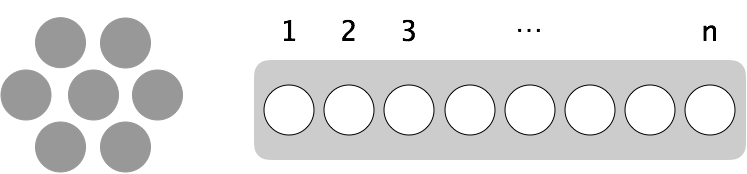
\includegraphics[scale=0.4]{FiguresMaths/GameTokenInit.png}
        \caption{Initial position: $n$ tokens (grey) and all the empty bank.}
        \label{fig:jeujetonsInit}
\end{center}
\end{figure}

The game consists in determining the process to fill the bank with the $n$ tokens, putting or removing one token at a time according to one of the two 
following constraints.
Both rules are illustrated in figures~\ref{fig:rule1} and \ref{fig:rule2}.

\begin{itemize}
\item \textbf{Rule 1.} Position 1: Put a token if it is empty or remove it.
\item \textbf{Rule 2.} Position next to the first empty position (i.e. on the right): Put a token if the position is empty or remove it.
\end{itemize}

Notice that the first rule only refers to positions (and thus, it is symmetric in regard to the move: put or remove a token), 
while the second one is not symmetric.

\begin{figure}[h]
\begin{center}
        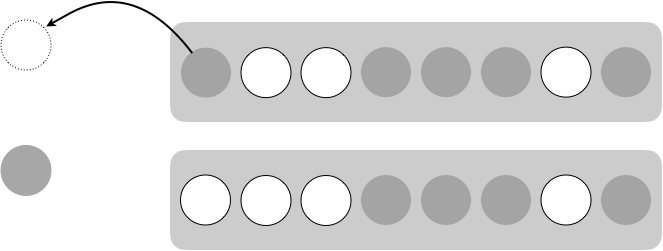
\includegraphics[scale=0.4]{FiguresMaths/GameTokenRule1.png}
        \caption{Rule 1: Position 1 contains a token, thus, remove it.}
        \label{fig:rule1}
\end{center}
\end{figure}

\begin{figure}[h]
\begin{center}
        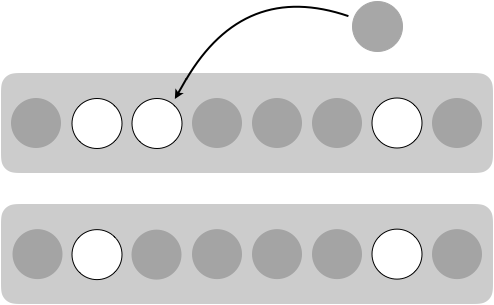
\includegraphics[scale=0.4]{FiguresMaths/GameTokenRule2.png}
        \caption{Rule 2: The position next to the first idle position (i.e. position 3 in this example) 
        is idle, thus, put a remaining token here.}
        \label{fig:rule2}
\end{center}
\end{figure}

The analysis of the game for some particular values of $n$ leads to some evidences (looking at the first ranks):
First, in the even case, the process should start by putting the second token while in the odd case, we should start to fill the first position.
%Then, the first token is flipped every double steps, the second one every four steps and so on.
Second observation: both rules are applied alternatively (this is obvious for Rule 1 since applying it twice consecutively leads to the initial position, 
and easy to check for Rule 2 on the first ranks). 
However, the solution is not easy to describe and its cost is not easy to establish.

The solution can be easily expressed recursively as follows (for $n > 2$):
the token in the last position can only be put bu rule 2, that means that the first $(n-2)$ one are on the bank.
Then, if we empty these first $n-2$ positions,
we obtain a configuration similar as in the initial one except for the last position which has a token. 
Then, the puzzle is solved by applying the same process on a bank with $n-1$ tokens.
The successive steps of this recursive solution are depicted in Figure~\ref{fig:jeujetonsPrinciple}.

%Thus, flipping the first tokens of the same color is different if they are all blue or red.
%Notice that flipping the first reds can be obtained using the reverse process as for the blue ones (see coding at the end of this document).

\begin{figure}[h]
\begin{center}
        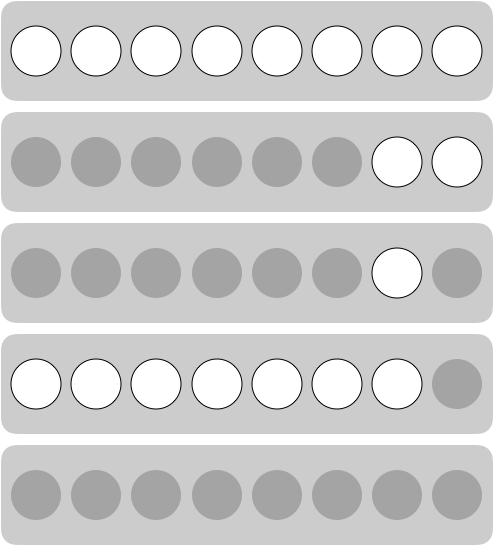
\includegraphics[scale=0.4]{FiguresMaths/GameTokenPrinciple.png}
        \caption{Principle of the recursive solution. Fill the bank in the $(n-2)$ first positions, then, put a token on the last position (Rule 2), 
        empty the (n-2) first positions. Finally, fill the $(n-1)$ first positions of the bank.}
        \label{fig:jeujetonsPrinciple}
\end{center}
\end{figure}
\bigskip

More formally,
\bigskip

fillBank(n)
\begin{itemize}
\item
 if $n=1$ then putToken(1) -- according to Rule 1
\item
if $n=2$ then PutToken(2) -- Rule 2 -- and then PutToken(1) -- Rule 1

\item 
if $n > 2$ then
\begin{itemize}
\item fillBank(n-2)
\item PutToken(n)
\item EmptyBank(n-2)
\item FillBank(n-1)
\end{itemize}
\end{itemize}

\subsection{Analysis}

The analysis comes directly from the previous process. 

Let call $f(i)$ the cost for filling the bank from position $1$ to position $i$
(the cost here refers to the number of elementary moves, put or remove a token).
Notice that it requires the same number of steps to fill or to empty the truncated bank (from position $1$ to $i$). 
The total cost is to fill the whole bank of size $n$, thus we have to solve:

$f(n) = f(n-2) + 1 + f(n-2) + f(n-1) = f(n-1) + 2.f(n-2) +1$ for $n > 2$

with $f(1) = 1$ and $f(2) = 2$.
\bigskip

If we add $f(n-1)$ in both sides of the previous expression, we obtain a simpler equation (call $s(n)$ the sum $f(n)+f(n-1)$ $n \geq 2$,
in particular, $s(2) = 2+1$):

$f(n) + f(n-1) = 2.f(n-1) + 2.f(n-2) +1$

$s(n) = 2.s(n-1)+1 = 2.(2.s(n-2)+1) + 1 = 2^2 s(n-2) + 2+ 1 = 2^3 s(n-3) + 2^2 + 2 + 1 = ... = 2^{n-2} s(2) + 2^{n-3} + ... + 2^2 + 2 + 1$ where $s(2) = 2+1$

$s(n) = 2^{n-1} + 2^{n-2} + 2^{n-3} + ... + 2^2 + 2 + 1$ 

Summing up this geometric series leads to
$s(n) = 2^{n} -1$
\bigskip

Coming back to the $f(n)$, we can rewrite this equation as:

$f(n) = 2^{n} - f(n-1) -1$ where $f(1)=1$

$f(n) = 2^{n} - 2^{n-1} + f(n-2) +1 -1 = 2^{n} - 2^{n-1} + 2^{n-2} - f(n-3) -1 = ...$

This sequence is an alternate series of the powers of $2$ where the $1$ and $-1$ are cancelled two by two.
However, there is a different number of steps if $n$ is even or not. 
In this case, the last term is $-2$, while it is $-1$ when $n$ is odd.
\bigskip

For $n$ even, $f(n) = \sum_{1 \leq k \leq n}(-1)^{k}2^{k} $

For $n$ odd, $f(n) = \sum_{0 \leq k \leq n}(-1)^{k+1}2^{k} $
\bigskip

$f(n)$ is an alternate series of the successive powers of $2$, which can be solved by a graphical proof.

We rewrite it by gathering the positive and negative terms as follows (for odd $n$): 
$f(n) = (2^{n} + 2^{n-2} + ... + 2) - (2^{n-1} + 2^{n-3} + ... + 1)$

$= 2.(2^{n-1} + 2^{n-3}  + ...  +1) - (2^{n-1} + 2^{n-3}  + ... + 1)$

$= 2^{n-1} + 2^{n-3}  + ...  +1$ 

Consider first the odd case (here, $2^{n+1}$ is a perfect square).
Figure~\ref{fig:alternatePowers2odd} gives a representation of $f(n)$ 
where the smallest surface at the right is the unit square.

Take 3 copies of $f(n)$ as it is depicted in figure~\ref{fig:alternatePowers2finalOdd},
two are mirror configurations and the third one (represented in grey) fills the remaining part of a big square but some idle space at the 2 extreme right corners. 
The whole surface is a perfect $2^{n} \times 2^{n}$ square, equal to $2^{n+1}$ plus the small surface equal to half of the basic unit square ($2 \times \frac{1}{2}$ = 1). Thus, $3.f(n)+1= 2^{n+1}$.

\begin{figure} [h]
\begin{center}
        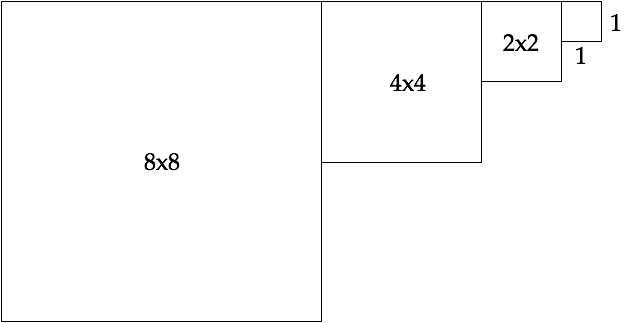
\includegraphics[scale=0.4]{FiguresMaths/alternatePowers2initOdd.png}
        \caption{Representation of the alternate series of powers of $2$ for $n=7$.
        f(7)=64+16+4+1.}
        \label{fig:alternatePowers2odd}
\end{center}
\end{figure}

\begin{figure} [h]
\begin{center}
        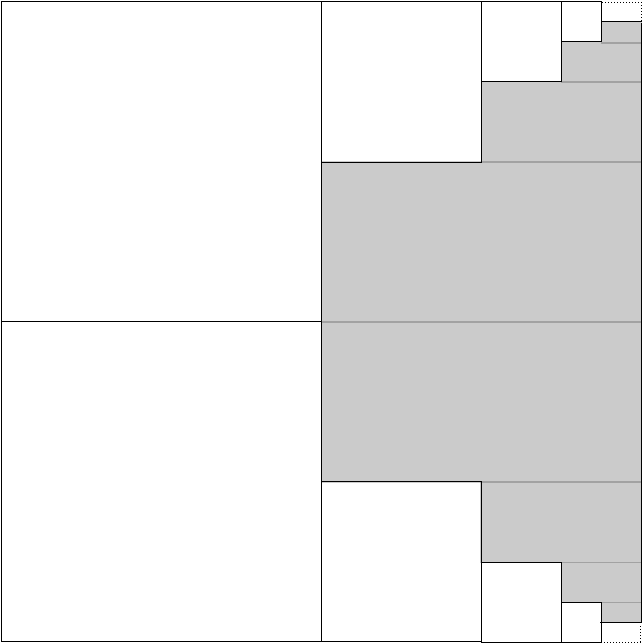
\includegraphics[scale=0.4]{FiguresMaths/alternatePowers2odd.png}
        \caption{Even case: Geometric proof using 3 copies of $f(n)$ that almost fill a large square.}
        \label{fig:alternatePowers2finalOdd}
\end{center}
\end{figure}

The previous construction may be adapted in the even case in a similar way.
The details are left to the readers. 

We propose below another proof obtained by using the results for the odd case:

We start by the expression $f(n) + f(n-1) = 2^n -1$
that is $f(2k) = 2^{2k} - f(2k-1) -1$ for even $n=2k$.

Now, apply the final expression of $f$ to $2k-1$, which is odd: $f(2k-1) = \frac{1}{3} (2^{2k+1}-1)$.

$f(2k) = 2^{2k} - \frac{1}{3} (2^{2k-1+1}-1) -1 = 2^{2k} (1-\frac{1}{3}) + \frac{1}{3} -1= \frac{1}{3} (2^{2k+1} -2)$.
\bigskip

%
%Figures~\ref{fig:alternatePowers2even} and~\ref{fig:alternatePowers2finalEven} illustrate the construction in the even case.
%The details are left to the readers. 
%We obtain $3.f(n)+2= 2^{n+1}$ by a similar analysis.
%However, we can deduce directly the even case from the odd case by remarking that $f(2k)=2.f(2k-1) +1$.
%
%This is obtained by the basic relations $f(n) = 2^{n} - f(n-1) -1$ and $f(2k-1) = \frac{1}{3} (2^{2k} -1)$.
%
%$n=2k$, $f(n) = 2^{2k} - \frac{1}{3} (2^{2k} -1) -1 = \frac{1}{3} (2^{n+1} -2)$.
%
%\begin{figure} [h]
%\begin{center}
%        \includegraphics[scale=0.4]{FIGmaths/alternatePowers2initEven.png}
%        \caption{Representation of the alternate series of powers of $2$ for $n=6$.
%        f(6)=32+8+2.}
%        \label{fig:alternatePowers2even}
%\end{center}
%\end{figure}
%
%
%\begin{figure} [h]
%\begin{center}
%        \includegraphics[scale=0.4]{FIGmaths/alternatePowers2even.png}
%        \caption{Case odd: Geometric proof in the odd case. Notice here that there are 2 small rectangles left at the extreme corners on the right,
%        whose surface is $1$ each.}
%        \label{fig:alternatePowers2finalEven}
%\end{center}
%\end{figure}

We finally obtain: 

$f(n) = \frac{1}{3} (2^{n+1} -1)$ if $n$ is odd.

$f(n) = \frac{1}{3} (2^{n+1} -2)$ if $n$ is even.
